%Nama Kelompok: Sistem_Operasi_Deadlock
%Kelas: D4 TI 1B
%Alit Fajar Kurniawan(1174057) 
%Muhammad Iqbal Panggabean(1174063)
%Muhammad Afra Faris(1174041)
%Khadijah Hasanah Puteri Harahap(1174044)

\section {USB TO SERIAL}

\subsection {Pengertian USB}
\subsubsection {Apa itu USB ?}
	Universal Serial Bus atau yang disingkat dengan USB adalah sebuah teknologi yang dapat memungkinkan para penggunanya untuk dapat menghubungkan hardware eksternal contohnya seperti printer, keyboard, harddisk, flashdisk dan perangkat keras lainnya. kecepatan trnasfer data yang didukung oleh USB sebesar 12 Mbps. pada saat ini semua PC sudah memiliki port USB sendiri minimal 2 buah port USB.

\subsection {Jenis-jenis usb}
\begin {enumerate}
\item
	USB 1.1 : Versi kabel USB 1.1 adalah versi yang pertama yang dirilis sekitar Agustus 1998 dan mulai banyak digunakan di berbagai perangkat elektronik. Versi original-nya, USB 1.0 tidak pernah digunakan pada perangkat elektronik. Versi kabel USB 1.1 ini Memiliki kecepatan up to 12 Mbps. logo yang di punyai oleh USB 1.1 ini berwarna biru dan simbol berbentuk trisula. Namun sekarang , Versi kabel USB ini sudah tidak digunakan lagi.
\item
	USB 2.0 : versi kabel USB 2.0 adalah versi yang kedua yang di rilis pada tahun 2000. Kabel usb ini memiliki kecepatan maximum up to 480Mbps dengan Hi-Speed mode atau pada Full-Speed mode memiliki kecepatan 12 Mbps . Kabel USB ini memiliki supply tegangan maximumnya ( max power out put ) adalah 2.5V, 1.8A dan akan tetap berfungsi baik jika dihubungkan dengan versi sebelumnya ( backward - compatible with USB 1.1 )
	
\subsection {Ada Beberapa Keistimewaan dari USB}
\begin {enumerate}
\item
 PC atau komputer dapat dijadikan sebagai sebuah host
\item
 127 perangkat atu lebih dapat terhubung ke PC atau komputer dengan menggunkan hub USb secara langsung
\item
 Jika menggunakan kabel USB secara langsung hanya bisa mencapai 5 meter dan apabila menggunakan perangkat hub dapat sampai 30 meter jangkauannya
\item
 Sifat perangkat USB 'hot swappable' yang artinya apabila ada perangkat keras yang telah menggunakan port USB sifatnya plug and play
\end {enumerate}	

\subsection {Cara menghubungkan USB flash disk dengan komputer}
	USB port digunakan oleh flash disk denga tujuan untuk dapat mnghubungkan dengan komputer. fungsi dari flash disk itu sendiri yaitu untuk dapat menyimpan data dan flash disk juga memiliki batas maksimal penyimpanan. Mempelajari tentang bagaimana cara menghubungkan flash disk dengan komputer merupakan hal yang sangat mudah karena kita hanya memasukkan flash disk kedalam port USB yang tersedia di PC atau komputer. Ini merupakan salah satu cara komunikasi antara komputer atau PC dengan hardware yng dihubungkan dengan komputer atau PC dan dilakukan melalui USB To Serial.
	
	\begin{figure}[ht]
	\centerline{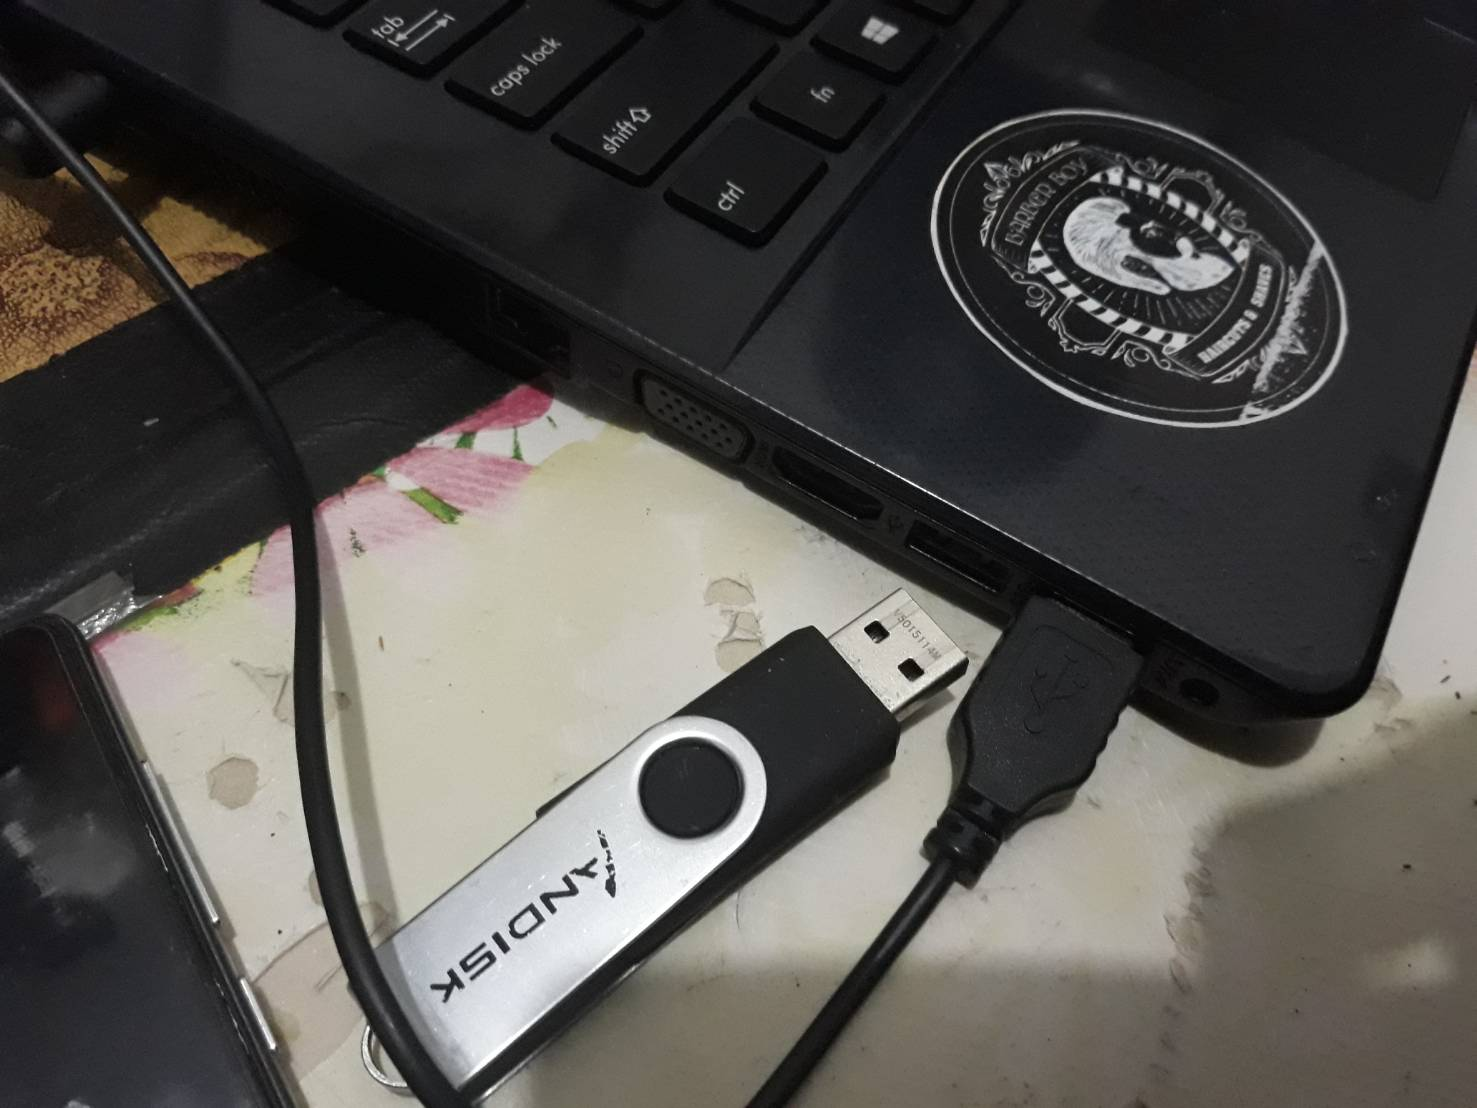
\includegraphics[width=1\textwidth]{figures/usb1.jpg}}
	\caption{Gambar memasukkan flash disk kedalam port usb pada PC}
	\label{Gambar}
	\end{figure}
      
      Gambar \ref{Gambar} Contoh gambar memasukkan flash disk kedalam port usb pada PC.
	  
\subsection {Beberapa istilah}	  
\begin{table}[H]
\begin{tabular}{|c|c|c|c|c|}
hline
No & Istilah & Arti dari Istilah\\
\hline
1   & Peripheral & Perangkat\\
2   & Hub & Sebuah alat yang digunakan untuk menghubungkan dan memperkuat sinyal dari satu PC dengan PC yang lain\\
3   & Plug and Play & Dapat langsung dikethui dan bisa digunakan oleh PC\\
4   & Port & Tempat untuk memasukkan USB\\
\hline
\end{tabular}
\end{table}


\subsection {Proses yang terjadi di USB}
	Ketika USB dimasukkan kedalam port USB pada komputer atau PC maka komputer atau PC akan mendata perangkat yang sudah tersambung ke port USB dan kemudian dilakukannya persiapan lamat memori kepada setiap perangkat yang terpasang. Proses ini disebut dengan enumerasi.
	
	\begin{figure}[ht]
	\centerline{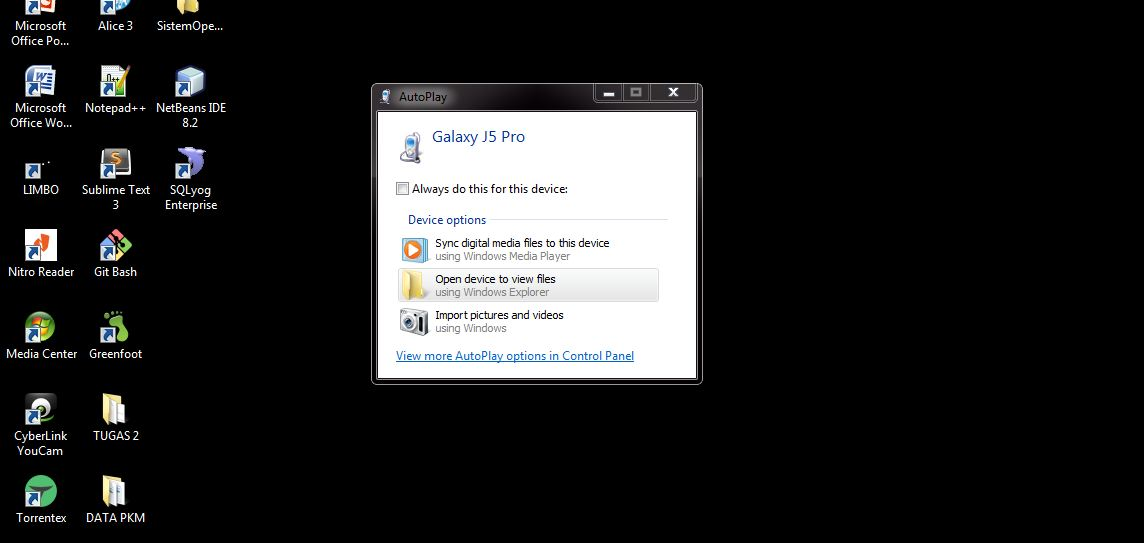
\includegraphics[width=1\textwidth]{figures/usb2.jpg}}
	\caption{Gambar proses enumerasi}
	\label{Gambar}
	\end{figure}
      
      Gambar \ref{Gambar} Contoh gambar proses enumerasi.
